% Set page numbering to arabic the first time we commence a chapter.
% This is required to get the page numbering correct.
\pagenumbering{arabic}

% Note that the text in the [] brackets is the one that will
% appear in the table of contents, whilst the text in the {}
% brackets will appear in the main thesis.

%% CHAPTER HEADER /////////////////////////////////////////////////////////////////////////////////////
\chapter[Introduction]{Introduction}
\label{ch:intro}
The dissertation results from the work of the author as an assistant in the Mechanics of Intelligent Structures Department, Institute of Fluid Flow Machinery, Polish Academy of Sciences.
Most of the work has been carried out within the framework of a research project, titled ‘Model-assisted damage identification function for Structural Health Monitoring of composite structures under a varied environmental condition’, which was awarded to the author by the National Science Centre.
The primary objective of the dissertation was to develop a new approach to a sandwich structure assessment based on guided waves techniques.
The essence of the proposed method is to establish an accurate and efficient numerical model of the wave propagation in the sandwich structure to determine the severity of the damage.
%% CHAPTER INTRODUCTION ///////////////////////////////////////////////////////////////////////////////

%% INCLUDE SECTIONS ///////////////////////////////////////////////////////////////////////////////////
%% SECTION HEADER /////////////////////////////////////////////////////////////////////////////////////
\section{Sandwich composite structure}
\label{sec:scs}

%% SECTION CONTENT ////////////////////////////////////////////////////////////////////////////////////
Composites consist of two or more different materials, such as plastics, resins, metal alloys, glass, carbon or bio-based fibres. The combination of material constituents gives  structure benefits from the properties of the component materials, e.g., the strength of carbon fibres and the low density of the polymer resin in the case of \ac{cfrp}.
The contribution of lightweight composite materials to the production of structural components has been increasing rapidly since the middle of the last century.
Composite materials are extensively used in aircraft, aerospace and civil constructions due to their high strength-to-weight ratio, high operating temperatures, great stiffness and high reliability.
For example, composites account for more than 50\% of the total weight of the aircraft Boeing 787 and Airbus A350 \cite{giurgiutiu2015structural}.

One group of composites includes sandwich panels, a multi-layered structure consisting of a mid-core attached between thin shells.
The skins, made of high-strength materials, are designed to carry tensile or compressive stresses from longitudinal forces and bending moments.
On the other hand, the core transmits mainly shear stresses from transverse forces.
It also separates the skins, which increases structural stiffness for thin layers, improves insulation properties, and reduces weight while maintaining strength properties similar to the solid construction of the same density.
A popular core used in engineering structures is a honeycomb geometry core. 
The typical \ac{hsc} is shown in Figure~\ref{fig:hcp}.
The core is composed of lightweight materials, the most common of which include aluminium, cardboard or Nomex\textsuperscript{\tiny\textregistered}.
\begin{figure}[H] %hbtp
	\begin{center}
		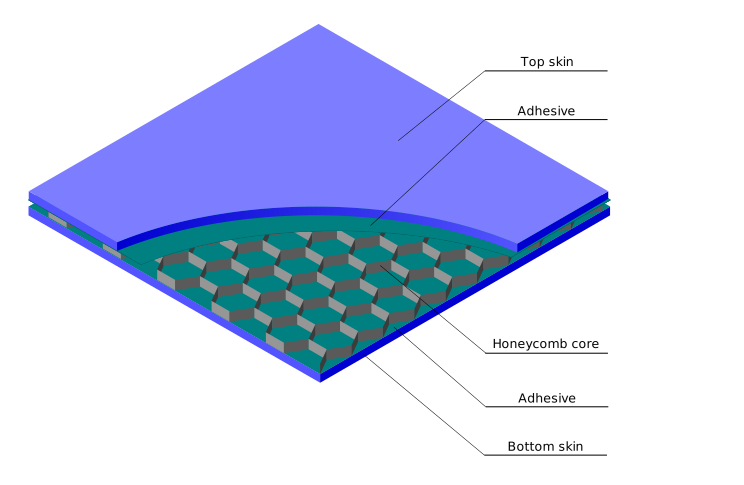
\includegraphics[width=0.95\textwidth]{Intro/honeycomb_plate}
		\caption{
			\label{fig:hcp} Structure of the honeycomb sandwich composite}
		\vspace{-0.5cm}
	\end{center}
\end{figure}

However, various types of damage can occur in these complex structures not found in metal alloy materials. These types of damage include hidden disbonds of the skin and core, delamination of composite skins, or impact damage to the core.
Damage can appear during manufacturing, storage, and operation, so online defect detection methods are required.
Therefore, the increased use of composite materials in the industry has motivated the development of advanced approaches to structural inspections, e.g., methods based on elastic wave propagation had to account for the anisotropic structure of the material.
%% SECTION HEADER /////////////////////////////////////////////////////////////////////////////////////
\section{Structural Health Monitoring}
\label{sec:scm}

%% SECTION CONTENT ////////////////////////////////////////////////////////////////////////////////////
\Ac{shm} is the process of implementing an advanced damage identification strategy for structural or mechanical systems \cite{farrar2007introduction}.
The \ac{shm} systems usually consist of a sensor network, a \ac{dau}, and a central processor.
The \ac{dau} is responsible for collecting the data measured by the sensor network and the intact structure data if used \ac{shm} technique requires it.
A central unit then determines the current state of the structure through signal processing and statistical classification.
\ac{shm} implementation aims to extend the safe life of equipment, use lightweight materials, and reduce manufacturing and operating costs.
For example, the use of composites and adhesive bonding techniques reduces the aircraft's overall weight, thereby reducing fuel consumption \cite{scelsi2011potential}.
\ac{shm} is most commonly found in structures, such as aerospace, civil and mechanical engineering, where damage can have catastrophic consequences.

In his dissertation \cite{rytter1993vibrational}, Rytter classified the \ac{shm} system advancement into the following four levels:
\begin{itemize}
	\item[] \textbf{Level 1}: Detection
	\item[] \textbf{Level 2}: Localization,
	\item[] \textbf{Level 3}: Assessment,
	\item[] \textbf{Level 4}: Consequence.
\end{itemize}
The first level determines if there has been an adverse change in the geometric or material characteristics of the system, and the second level leads to localization of the damage.
The third and fourth level systems determine the size of the flaw and decide whether any maintenance is necessary, respectively.
While existence and location identification can be performed without knowledge of the intact state of the structure, the two last levels require a supervised learning mode \cite{worden2007fundamental}.
%% SECTION HEADER /////////////////////////////////////////////////////////////////////////////////////
\section{Piezoelectric Transducers}
\label{sec:PZT}

%% SECTION CONTENT ////////////////////////////////////////////////////////////////////////////////////
The piezoelectric phenomenon is the generation of an electrical charge on the surface of materials under mechanical deformation in crystalline materials with no inversion symmetry.
The magnitude of the generated charge is proportional to the strain and the direction of polarization.
Those materials also exhibit the opposite effect: a change in size due to an applied electric field.
Piezoelectric materials are widely used in engineering as electroacoustic transducers, high voltage generators and power sources, energy harvesters, micro motors and actuators.
\begin{figure}[H]
	\begin{center}
		\includegraphics{Intro/PZTs}
	\end{center}
	\caption{Various types of piezoelectric transducers \textbf{(a)} circular discs, \textbf{(b)} circular array of the transducers, \textbf{(c)} Smart Layer\textsuperscript{\tiny\textregistered} sensors - piezoelectrics embedded into dielectric film manufactured by Acellent Technologies, Inc.}
	\label{fig:piezo}
\end{figure}
\Acp{pzt}, the acronym derived from the chemical formula of the most commonly used piezoelectric ceramic, i.e. Pb[Zr\(_x\)Ti\(_{1-x}\)]O\(_3\) (lead zirconate titanate), are lightweight, various size and shape structures. 
They can be permanently mounted on the structure surface, embedded within the material, or even be a smart composite material.
In \ac{shm}, they are mainly used in elastic wave propagation, modal analysis, and \ac{emi} methods.
%% SECTION HEADER /////////////////////////////////////////////////////////////////////////////////////
\section{Challenges in Damage Assessment in the SCS}
\label{sec:challenges}

%% SECTION CONTENT ////////////////////////////////////////////////////////////////////////////////////


%% SECTION HEADER /////////////////////////////////////////////////////////////////////////////////////
\section{Conclusions}
\label{sec:conclusionsIntro}

%% SECTION CONTENT ////////////////////////////////////////////////////////////////////////////////////
In the Introduction, a brief overview of the issues undertaken in the dissertation has been presented,  i.e., composite materials, construction and their applications;  definition of the \ac{shm} and application of \ac{pzt} sensors in damage detection; and challenges in severity damage assessment in \acp{hsc}.
The literature review revealed the need for a practical tool for damage size estimation in \acp{hsc} to fully exploit composites advantages in engineering structures.